\section{Caracterización de datos de trayectorias individuales}
\label{sec:caracterizacion}
El análisis de datos comienza con una etapa fundamental: la caracterización del conjunto de datos. Esta fase tiene como objetivo examinar y comprender la estructura, el contenido y las principales propiedades de los datos antes de aplicar técnicas analíticas más complejas. 

En el caso de los datos de trayectorias individuales, la caracterización permite identificar posibles inconsistencias, redundancias y elementos irrelevantes que puedan afectar la calidad del análisis. Las tareas principales llevadas a cabo en esta etapa son las siguientes:
\begin{itemize}
    \item Explorar las primeras filas del conjunto de datos para obtener una visión general de su estructura.
    \item Verificar la cantidad total de registros y columnas disponibles.
    \item Identificar y eliminar columnas que no aportan información relevante para el análisis o inconsistentes.
    \item Identificar y eliminar las filas que no aportan información relevante para el análisis o inconsistentes.
\end{itemize}
A continuación, se describen en detalle las acciones específicas realizadas durante el proceso de caracterización.


\subsection{Exploración inicial del conjunto de datos}
\label{subsec:exploracion_inicial}

Como primer paso en la caracterización, se realizó una exploración preliminar del conjunto de datos con el fin de comprender su estructura general. Para ello, se inspeccionaron las primeras dos filas, lo cual permitió identificar las columnas presentes y observar ejemplos representativos de sus valores.

El código utilizado para realizar esta exploración se encuentra en el Apéndice \ref{cod:csv_glance}. A continuación, se presenta un resumen de las columnas detectadas junto con una muestra de sus respectivos valores:

\begin{enumerate}[leftmargin=*, align=left, noitemsep]
    \item \texttt{id}: Identificador numérico único para cada registro. Ejemplo: \texttt{['34284565','34284566']}.
    \item \texttt{identifier}: Identificador único del dispositivo.  
    \begin{small}
    \texttt{['f2640430-7e39-41b7-80bb-3fddaa44779c', 'f2640430-7e39-41b7-80bb-3fddaa44779c']}.
    \end{small}

    \item \texttt{identifier\_type}: Tipo de identificador del dispositivo; en este caso, \texttt{'gaid'} (Google Advertising ID para Android). Otros posibles valores incluyen \texttt{'idfa'} (Apple) o \texttt{'imei'}.  
    Ejemplo: \texttt{['gaid', 'gaid']}.

    \item \texttt{timestamp}: Fecha y hora del registro de movilidad.  
    Ejemplo: \texttt{['2022-11-07 02:04:21', '2022-11-08 17:29:35']}.

    \item \texttt{device\_lat/device\_lon}: Coordenadas geográficas (latitud y longitud) del dispositivo.  
    Ejemplo: \texttt{['21.843149', '21.843149']}, \texttt{['-102.196838', '-102.196838']}.

    \begin{small}
    \item \texttt{country\_short/province\_short}: Código del país (e.g., \texttt{MX}) y subdivisión administrativa (e.g., \texttt{MX.01} para Aguascalientes).  
    Ejemplo: \texttt{['MX', 'MX']}, \texttt{['MX.01', 'MX.01']}.

    \item \texttt{ip\_address}: Dirección IP del dispositivo en formato IPv6.  
    Ejemplo: \texttt{['2806:103e:16::', '2806:103e:16::']}.
    \end{small}

    \item \texttt{device\_horizontal\_accuracy}: Precisión estimada del GPS en metros (valores menores indican mayor precisión).  
    Ejemplo: \texttt{['8.0', '8.0']}.

    \begin{small}
    \item \texttt{source\_id}: Hash que representa la fuente de los datos, ya sea una aplicación o un dispositivo.  
    Ejemplo: \texttt{['449d086d...344', '449d086d...344']}.

    \item \texttt{record\_id}: Identificador único para cada registro de movilidad, diferente de \texttt{id}.  
    Ejemplo: \texttt{['77d795df...', '8f8e1281...']}.

    \item \texttt{home\_country\_code}: Código del país de residencia del usuario.  
    Ejemplo: \texttt{['MX', 'MX']}.

    \item \texttt{home\_geog\_point/work\_geog\_point}: Coordenadas geográficas del hogar y del lugar de trabajo en formato WKT (Well-Known Text).  
    Ejemplo: \texttt{['POINT(-102.37038 22.20753)', 'POINT(-102.37038 22.20753)']}.
    \end{small}

    \item \texttt{home\_hex\_id/work\_hex\_id}: Identificadores hexagonales del hogar y del trabajo, en una cuadrícula geoespacial (p. ej., H3).  
    Ejemplo: \texttt{['85498853fffffff', '85498853fffffff']}.

    \item \texttt{data\_execute}: Fecha en que el registro fue procesado (puede diferir de la fecha de recolección).  
    Ejemplo: \texttt{['2023-05-30', '2023-05-30']}.

    \item \texttt{time\_zone\_name}: Zona horaria del dispositivo.  
    Ejemplo: \texttt{['America/Mexico\_City', 'America/Mexico\_City']}.
\end{enumerate}


\newpage
\subsection{Dimensiones del conjunto de datos}
\label{subsec:dimensiones}
\noindent Se verificó el número total de registros y columnas en el conjunto de datos utilizando el siguiente código:

    \begin{lstlisting}[
        language=Python,
        caption={csv\_count\_registers.py, conteo de registros en el conjunto de datos.},
        label={cod:csv_count}
        ]
        import dask.dataframe as dd

        ruta_archivo = "Mobility_Data.csv" 
        columnas_usar = ["id"]  

        ddf = dd.read_csv(
            ruta_archivo,
            usecols=columnas_usar, 
            sep=",",             
            dtype={"id": "str"},  
            blocksize="256MB",   
        )

        print("Contando registros (paciencia para archivos grandes)...")
        total_registros = ddf.shape[0].compute() 

        print(f" Total de registros: {total_registros:,}")
    \end{lstlisting}

\noindent El resultado de la ejecución de este código es que el conjunto de datos contiene un total de 69,980,000 registros y 19 campos. Esto indica que hay una cantidad significativa de datos disponibles para el análisis.

\subsection{Depuración de columnas}
\label{subsec:depuracion_columnas}
\noindent Ya que tenemmos un conjunto de datos con 19 campos, es importante identificar y eliminar aquellas que no aportan valor al análisis. Para ello, vamos a revisar los valores únicos de los siguiente campos, para determinar si son redundantes o no aportan información relevante. A continuación, se presentan los campos que se consideran innecesarios:
\begin{itemize}
    \item \texttt{id}
    \item \texttt{identifier\_type}
    \item \texttt{country\_short}
    \item \texttt{province\_short}
    \item \texttt{ip\_address}
    \item \texttt{source\_id}
    \item \texttt{home\_country\_code}
    \item \texttt{home\_geog\_point}
    \item \texttt{work\_geog\_point}
    \item \texttt{home\_hex\_id}
    \item \texttt{work\_hex\_id}
    \item \texttt{data\_execute}
\end{itemize}

\noindent Para eliminar estos campos vamos a tomar solamente las columnas que sí vamos a conservar. A continuación, se muestra el código utilizado para realizar esta tarea:

    \begin{lstlisting}[
        language=Python,
        caption={remove\_columns.py, eliminación de campos innecesarios en el conjunto de datos.},
        label={cod:csv_slim}
        ]
        import dask.dataframe as dd

        # Columnas que si vamos a conservar
        columnas_deseadas = [
            'identifier',
            'timestamp',
            'device_lat',
            'device_lon',
            'device_horizontal_accuracy',
            'record_id',
            'time_zone_name'
            ]

        # Cargar solo las columnas necesarias
        df = dd.read_csv('Mobility_Data.csv', usecols=columnas_deseadas)

        # Guardar el resultado
        df.to_csv('Mobility_Data_Slim.csv', index=False, single_file=True, encoding='utf-8-sig')
    \end{lstlisting}

\noindent El resultado de la ejecución de este código es un nuevo archivo CSV que se guarda en la misma carpeta el cual contiene únicamente las columnas seleccionadas, eliminando así las que no aportan valor al análisis. 

\newpage
\subsection{Depuración de filas}
\label{subsec:depuracion_filas}
\noindent Ahora que tenemos una base datos más ligera, es importante identificar y eliminar las filas que no aportan valor al análisis. Para ellos, vamos a realizar diagramas que nos permitan identificar la distribución de los datos y poder determinar si hay filas que no aportan valor al análisis. Las tablas seleccionadas para este análisis son las siguientes:
\begin{itemize}
    \item \texttt{identifier}: Identificador único del dispositivo.
    \item \texttt{device\_horizontal\_accuracy}: Precisión del GPS en metro. Menor valor = mayor precisión. 
\end{itemize}

\noindent La primer columna analizada fue \texttt{device\_horizontal\_accuracy}, que representa la precisión del GPS en metros. Estos valores dependen del sistema de medición y la fuente de los datos, generalemente se sigue la siguiente escala:
\begin{itemize}
    \item GPS puro (satelital): 1-20 metros.
    \item A-GPS (Asistido por red): 5-50 metros.
    \item Triangulación por WiFi/redes móviles: 20-500 metros.
    \item Geolocalización por IP: 1000-5000 metros.
\end{itemize}

\noindent Con base en esta escala, el primer paso es identificar el rango de valores que contiene la columna. Para ello, se utilizó el \textit{Código:} \ref{cod:unique_values}, que permite obtener los valores únicos de la columna \texttt{device\_horizontal\_accuracy} y guardarlos en un archivo de texto. 

    \begin{lstlisting}[
        language=Python,
        breaklines=true,
        caption={unique\_values.py, obtención de valores únicos de la columna 'device\_horizontal\_accuracy'.},
        label={cod:unique_values}
        ]
        import dask.dataframe as dd
        import pandas as pd
        from tqdm import tqdm

        archivo_csv = "Mobility_Data.csv" 
        columna_objetivo = "device_horizontal_accuracy"  
        archivo_salida = "valores_unicos.txt"
        chunksize = 1_000_000  # Procesar 1M de registros a la vez

        valores_unicos = set()

        for chunk in tqdm(pd.read_csv(archivo_csv, usecols=[columna_objetivo], chunksize=chunksize)):
            valores_unicos.update(chunk[columna_objetivo].dropna().astype(str)) 

    
        with open(archivo_salida, "w", encoding="utf-8") as f:
            f.write("\n".join(sorted(valores_unicos)))  

        print(f"\n Se encontraron {len(valores_unicos):,} valores unicos.")
        print(f" Guardados en: {archivo_salida}")

        print("\n Ejemplo de valores unicos:")
        print("\n".join(sorted(valores_unicos)[:10]))
    \end{lstlisting}

\noindent Una vez obtenidos los valores únicos pudimos determinar que el rango de valores es de 0 a 200. Este rango es muy importante para poder crear un script que grafique los valores de la columna \texttt{device\_horizontal\_accuracy} y que nos permita identificar la frecuencia de los valores para poder determinar si hay filas que no aportan valor al análisis. Este script se muestra en el \textit{Código:} \ref{cod:accuracy_histogram}.

    \begin{lstlisting}[
        language=Python,
        caption={accuracy\_histogram.py, creación de un histograma de frecuencias de la columna 'device\_horizontal\_accuracy'.},
        label={cod:accuracy_histogram}
        ]
        import os
        import pandas as pd
        import matplotlib.pyplot as plt
        import numpy as np

        archivo_csv = "Mobility_Data_Slim.csv"
        columna = "device_horizontal_accuracy"  
        bins = 100 
        os.makedirs("img", exist_ok=True) 

        frecuencias = pd.Series(dtype=float)
        for chunk in pd.read_csv(archivo_csv, usecols=[columna], chunksize=1_000_000):
            frecuencias = pd.concat([frecuencias, chunk[columna].value_counts()])

        counts, edges = np.histogram(frecuencias.index, bins=bins, weights=frecuencias.values)

        plt.figure(figsize=(12, 6))
        plt.bar(edges[:-1], counts, width=np.diff(edges), align='edge', edgecolor='black', alpha=0.7)
        plt.title("Frecuencias de Valores Agrupados por Rangos (0-200)")
        plt.xlabel("Rango de Valores")
        plt.ylabel("Frecuencia Total (Millones)")
        plt.xticks(edges[::5], rotation=45) 
        plt.grid(axis='y', linestyle='--')

        output_path = "img/histograma_frecuencias_rangos.png"
        plt.savefig(output_path, dpi=300, bbox_inches='tight')
        plt.close()
    \end{lstlisting}

\noindent El resultado de la ejecución del script anterior es un histograma que muestra la frecuencia de los valores agrupados por rangos. En la siguiente figure se puede observar que la mayoría de los valores se encuentran en el rango de 0 a 20 metros, lo cual es consistente con la precisión del GPS puro. Con base en esto podemos acotar los valores que serán considerados válidos para el análisis.

\begin{figure}[H]
    \centering
    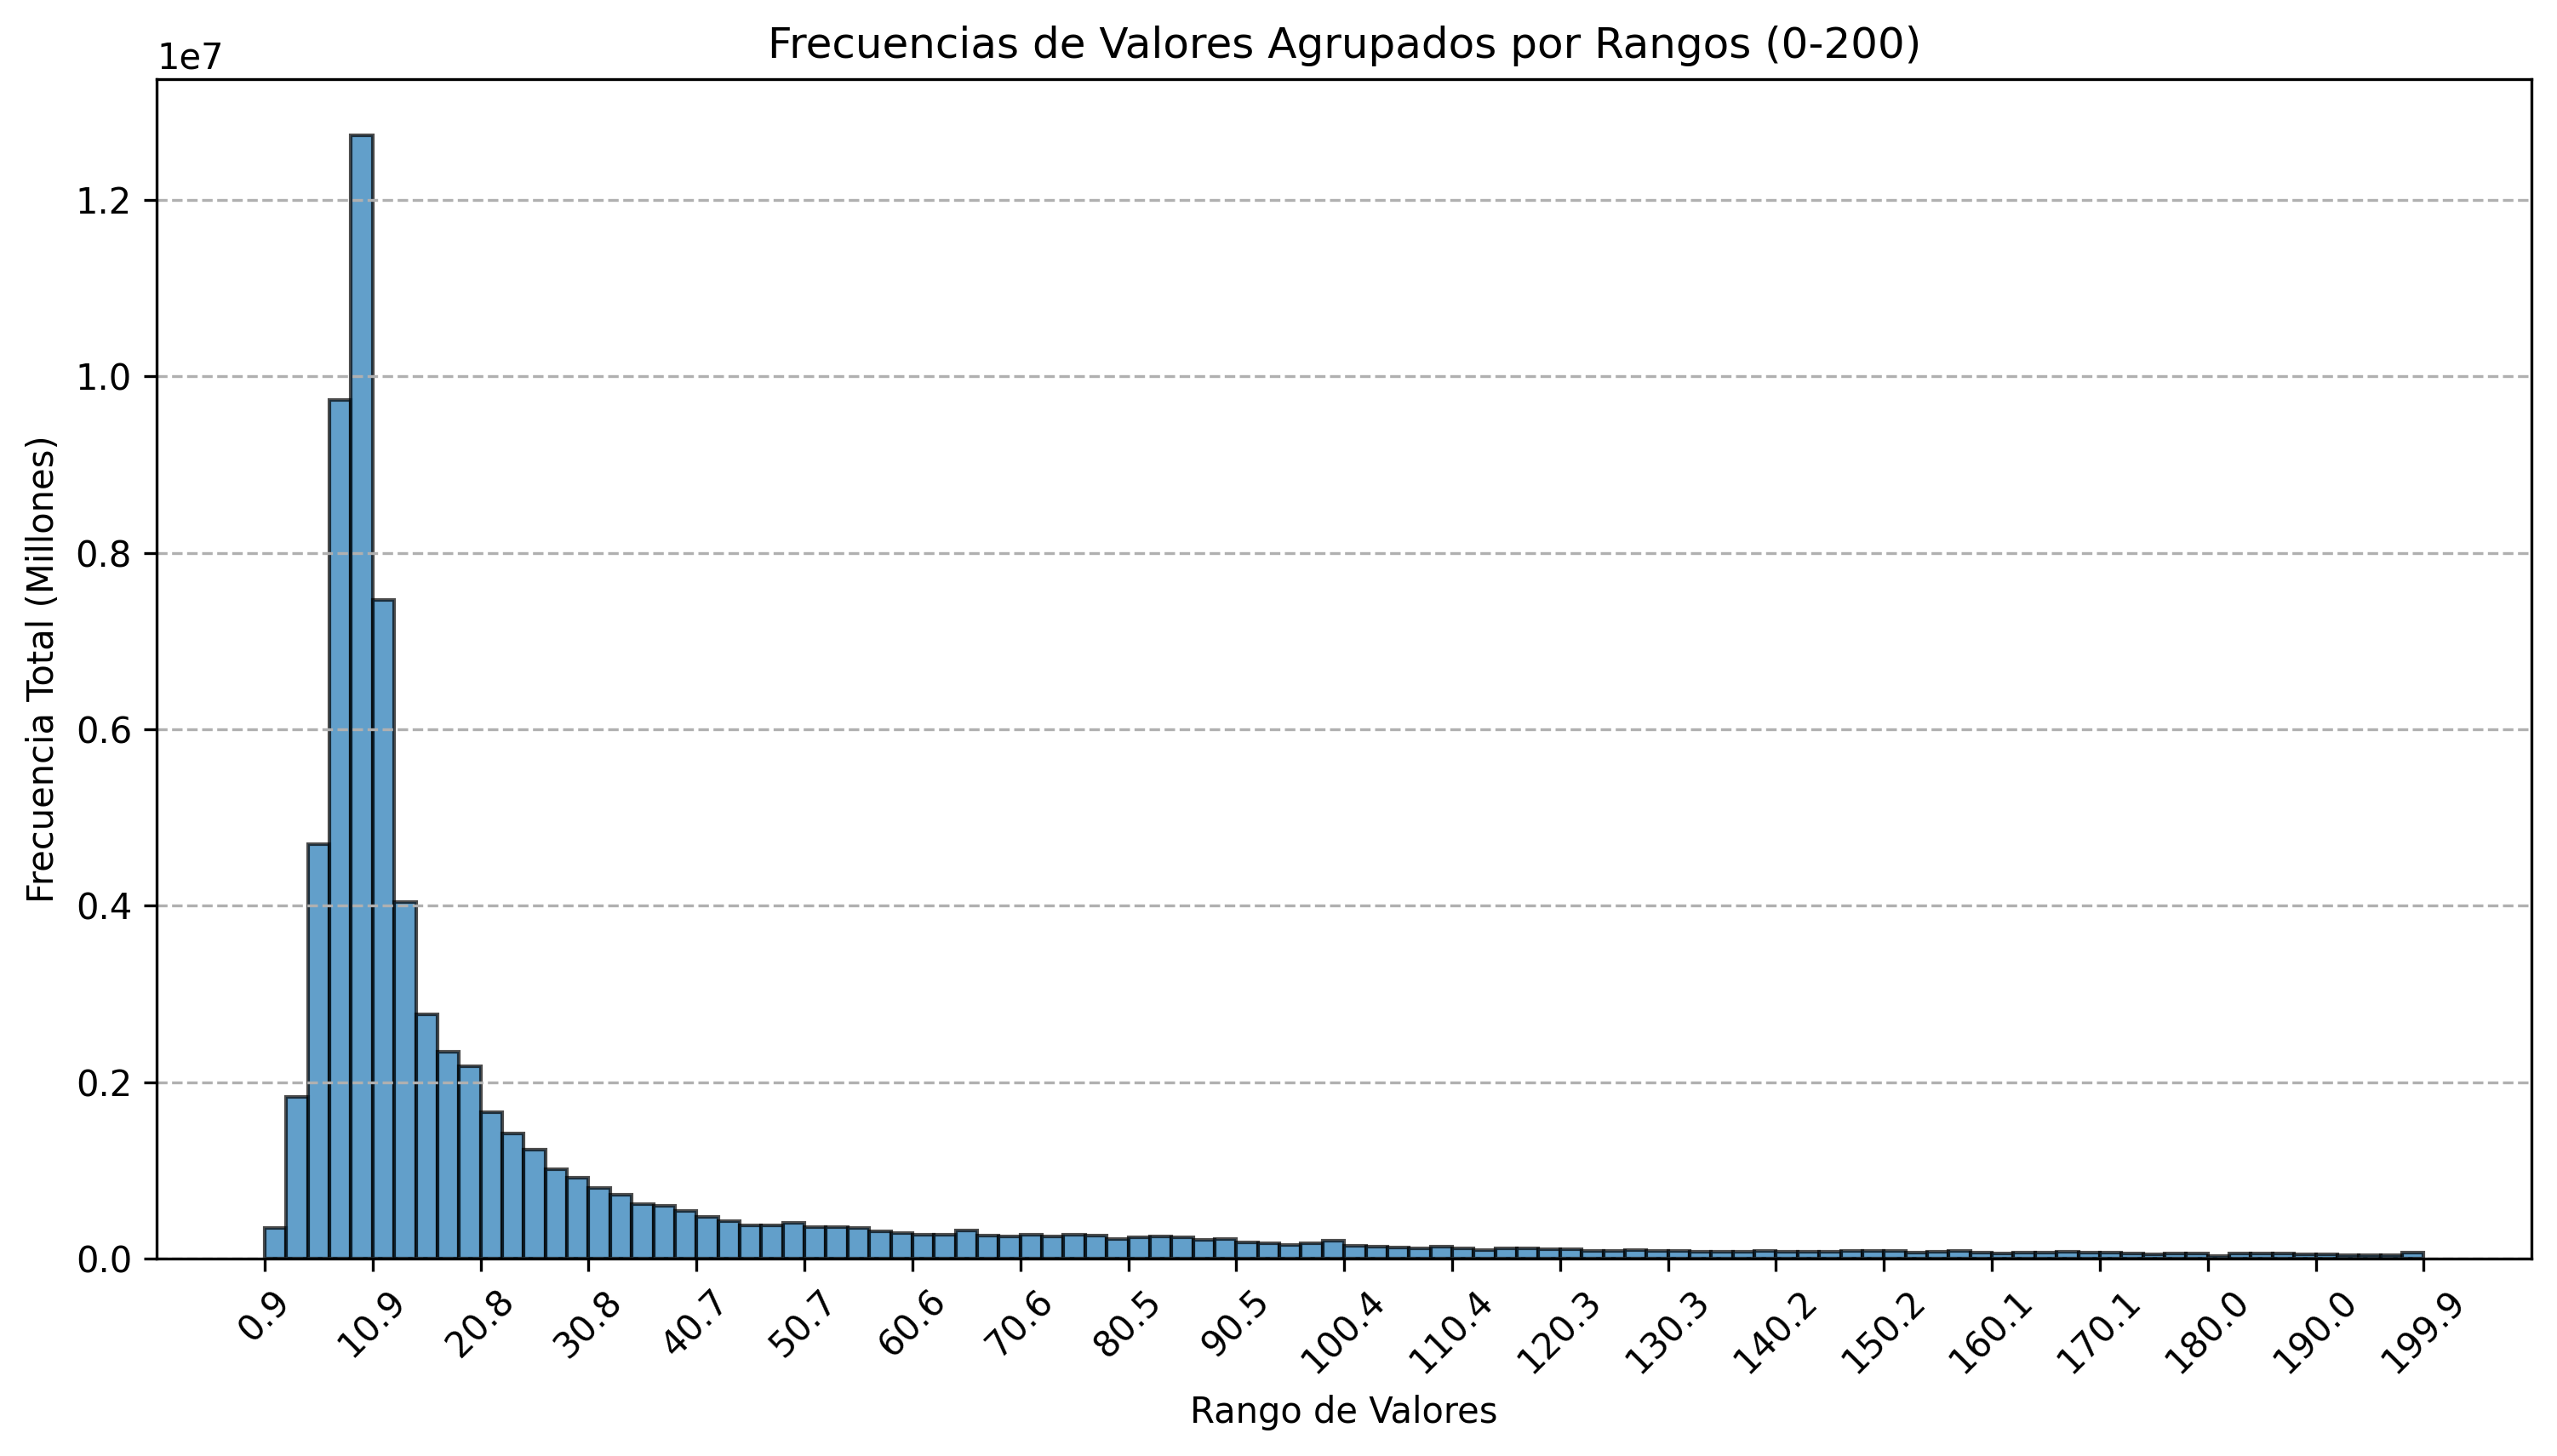
\includegraphics[width=\textwidth]{img/histograma_frecuencias_accuracy.png}
    \caption{Frecuencias de valores agrupados por rangos (0-200).}
    \label{fig:accuracy_histogram}
\end{figure}

\noindent Para poder tomar una mejor decisión sobre los valores que serán considerados válidos para el análisis, se realizó un conteo de los valores respecto a los rangos de precisión del GPS. 

\begin{itemize}
    \item GPS puro, satelital (1-20 metros): 68.73\%.
    \item A-GPS, asistido por red (5-50 metros): 16.56\%.
    \item Triangulación por WiFi/redes móviles (20-500 metros): 14.69\%.
\end{itemize}

\newpage

\noindent La siguiente columna analizada fue \texttt{identifier}, la cual representa el identificador único del dispositivo. El primer paso de este análisis es identificar la distribución de los valores únicos. Para ello, se utilizó un código que crea un gráfico que separa por intervalos el número de repeticiones, y pone la cantidad de valores único de forma logarítimica. 

\begin{lstlisting}[
    language=Python,
    caption={identifier\_histogram.py, creación de un histograma de frecuencias de la columna 'identifier'.},
    label={cod:identifier_histogram}
    ]
    import os
    import pandas as pd
    import matplotlib.pyplot as plt
    import numpy as np
    from collections import Counter

    archivo_csv = "Mobility_Data_Slim.csv"
    columna = "identifier"  
    chunksize = 1_000_000  
    os.makedirs("img", exist_ok=True) 

    counter = Counter()
    for chunk in pd.read_csv(archivo_csv, usecols=[columna], chunksize=chunksize):
        counter.update(chunk[columna].dropna().astype(str))

    frecuencias = pd.Series(counter)

    max_freq = frecuencias.max()
    bins = [0] + [10**i for i in range(0, int(np.log10(max_freq)) + 2)]  # Ej: [0, 1, 10, 100, 1000, ...]
    frecuencias_agrupadas = pd.cut(frecuencias, bins=bins, right=False).value_counts().sort_index()

    plt.figure(figsize=(12, 7))
    frecuencias_agrupadas.plot(kind='bar', logy=True, alpha=0.7, edgecolor='black')

    plt.xticks(rotation=45, ha='right')  # Rotar etiquetas para mejor legibilidad
    plt.title("Distribucion de Frecuencias Agrupadas en Bloques de 1000 Repeticiones")
    plt.xlabel("Rango de repeticiones (ej: [0, 1000) significa 0-999 repeticiones)")
    plt.ylabel("Cantidad de valores unicos (log)")
    plt.grid(True, which="both", ls="--", axis='y')

    output_path = os.path.join("img", "histograma_frecuencias_agrupadas_1000.png")
    plt.savefig(output_path, dpi=300, bbox_inches='tight')
    plt.close()
\end{lstlisting}

\begin{figure}[H]
    \centering
    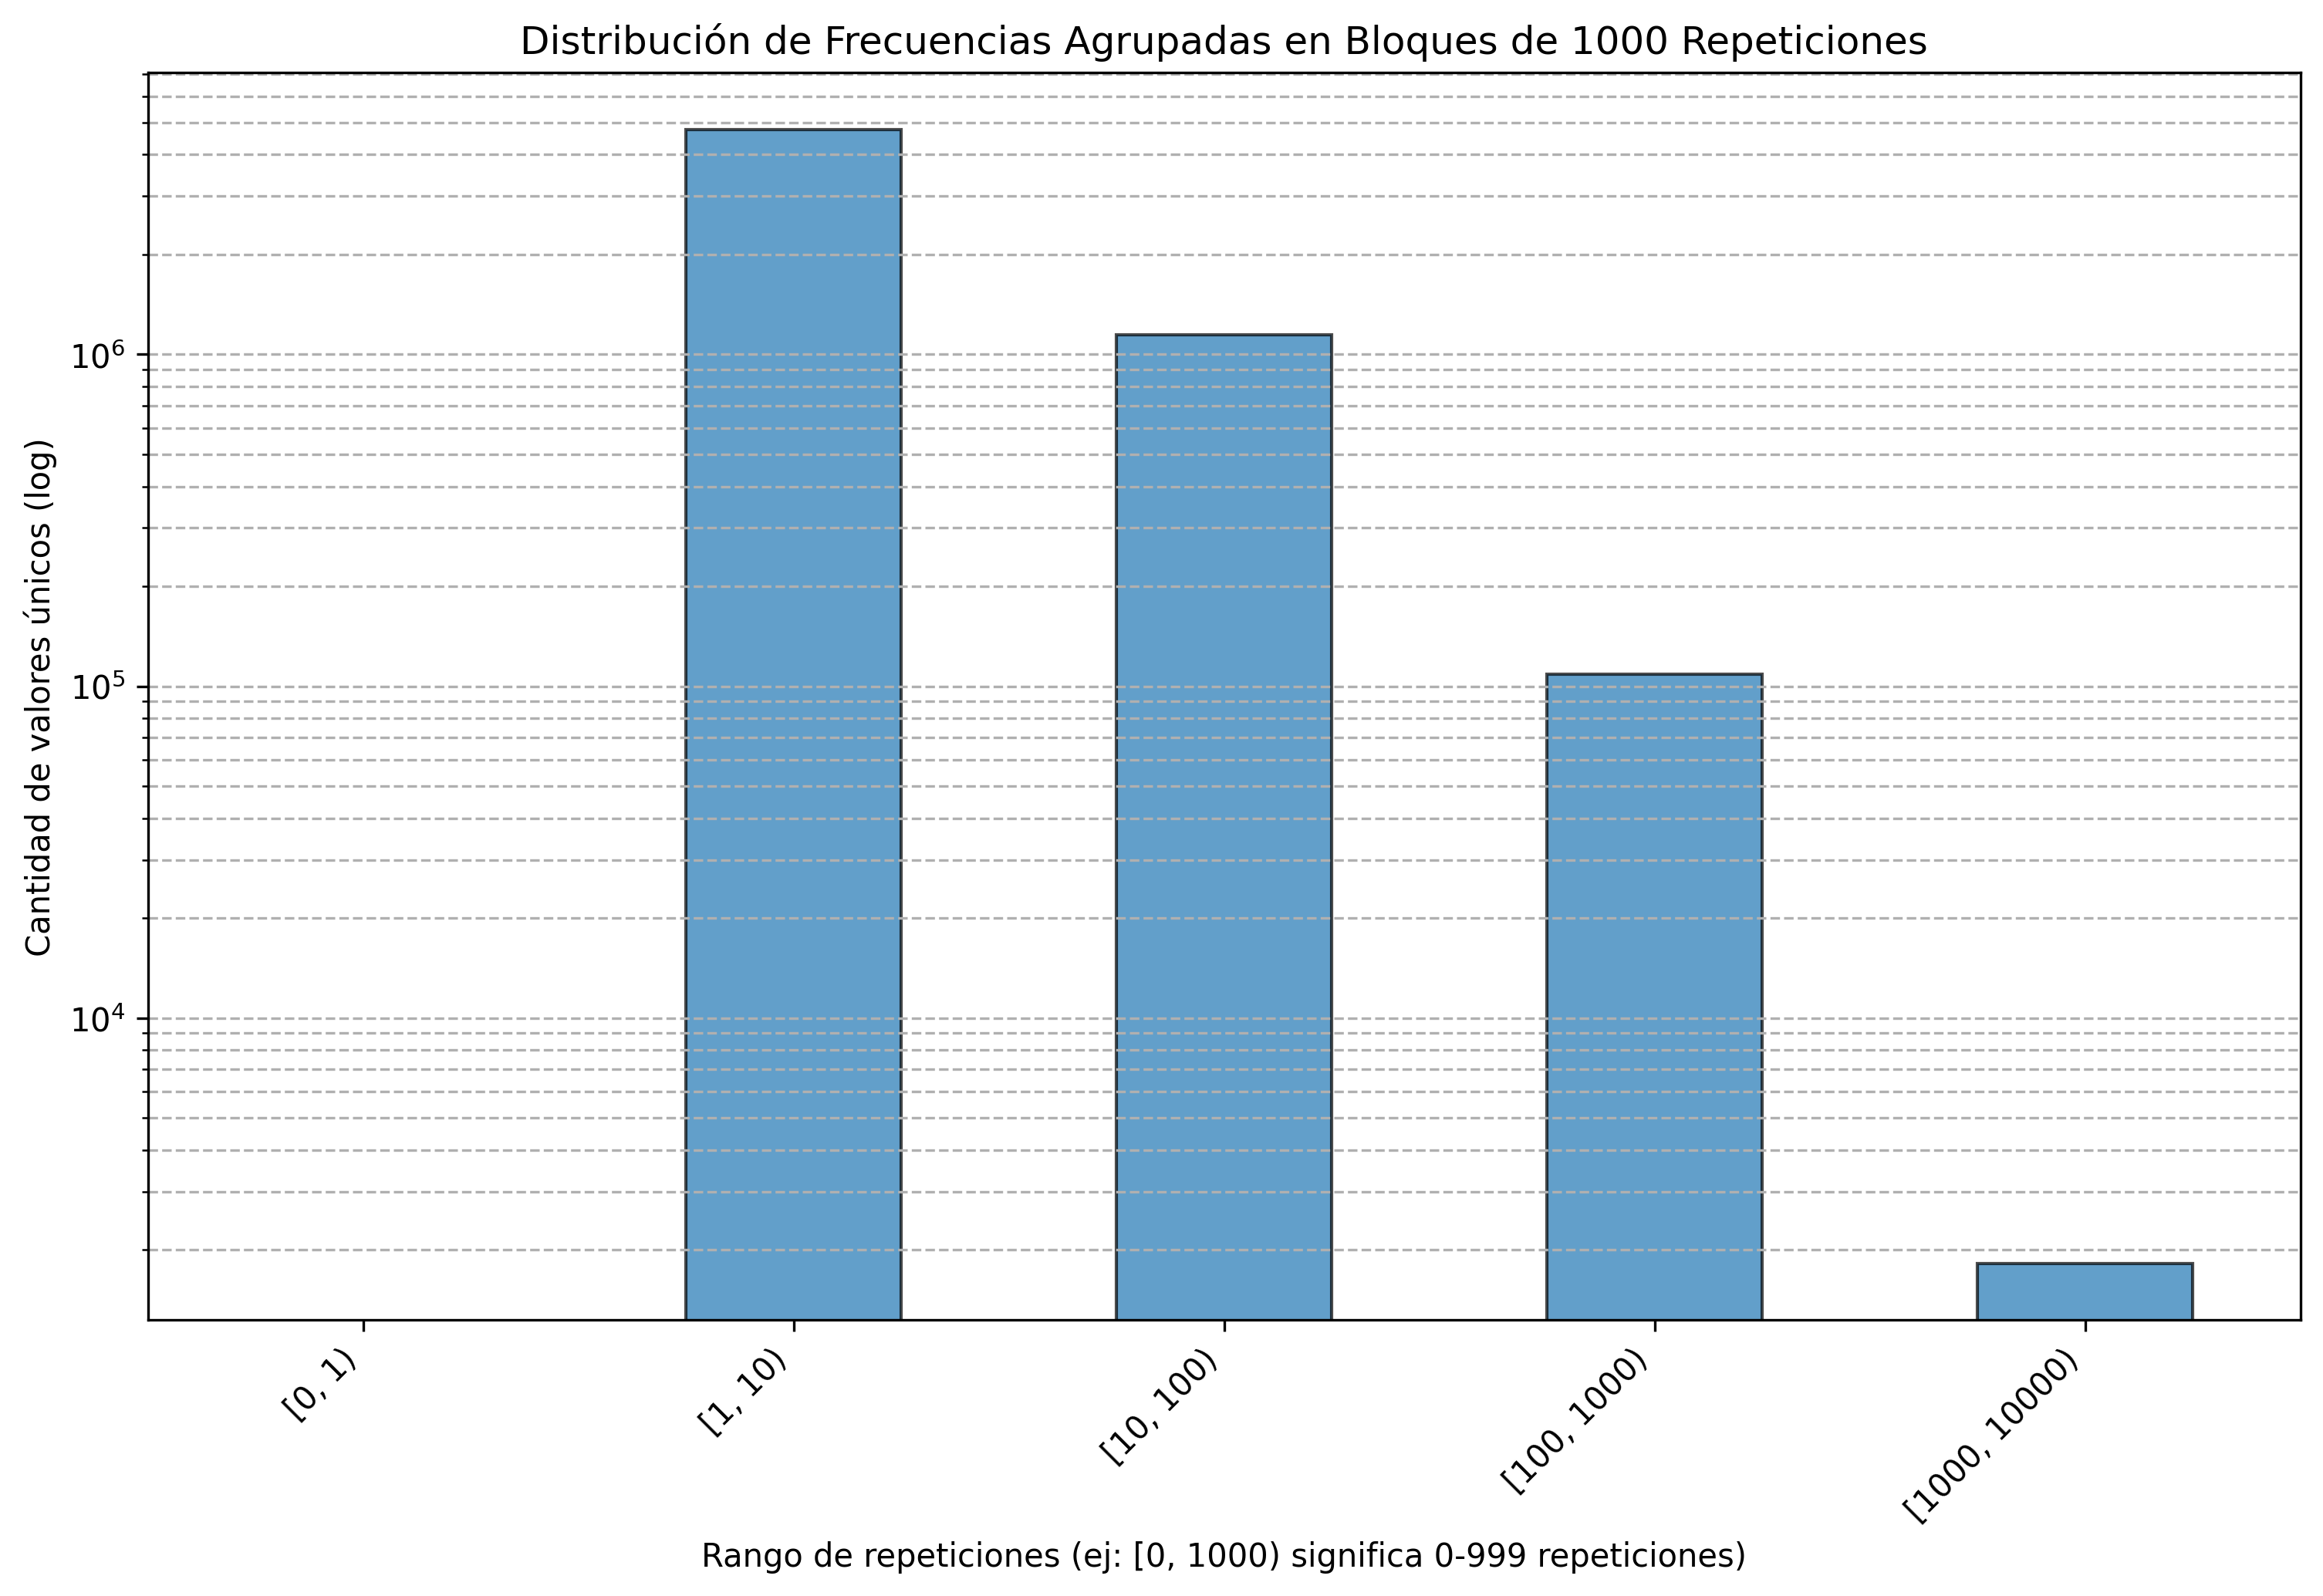
\includegraphics[scale=0.5]{img/histograma_frecuencias_agrupadas_1000.png}
    \caption{Distribución de frecuencias agrupadas en bloques de 1000 repeticiones.}
    \label{fig:identifier_histogram}
\end{figure}

\noindent Gracias a la \textit{Figura:} \ref{fig:identifier_histogram} podemos observar la frecuencia de los valores únicos. Para poder obtener información más detallada, usaremos el \textit{Código:} \ref{cod:identifier_histogram_detailed}. Este código nos permite obtener un análisis más detallados, separando los valores en tres rangos: 1-100, 100-1000 y 1000-10000.  

\begin{figure}[htbp]
    \centering
    \begin{subfigure}[t]{0.48\textwidth-1em} % Restamos 1em para el espacio
        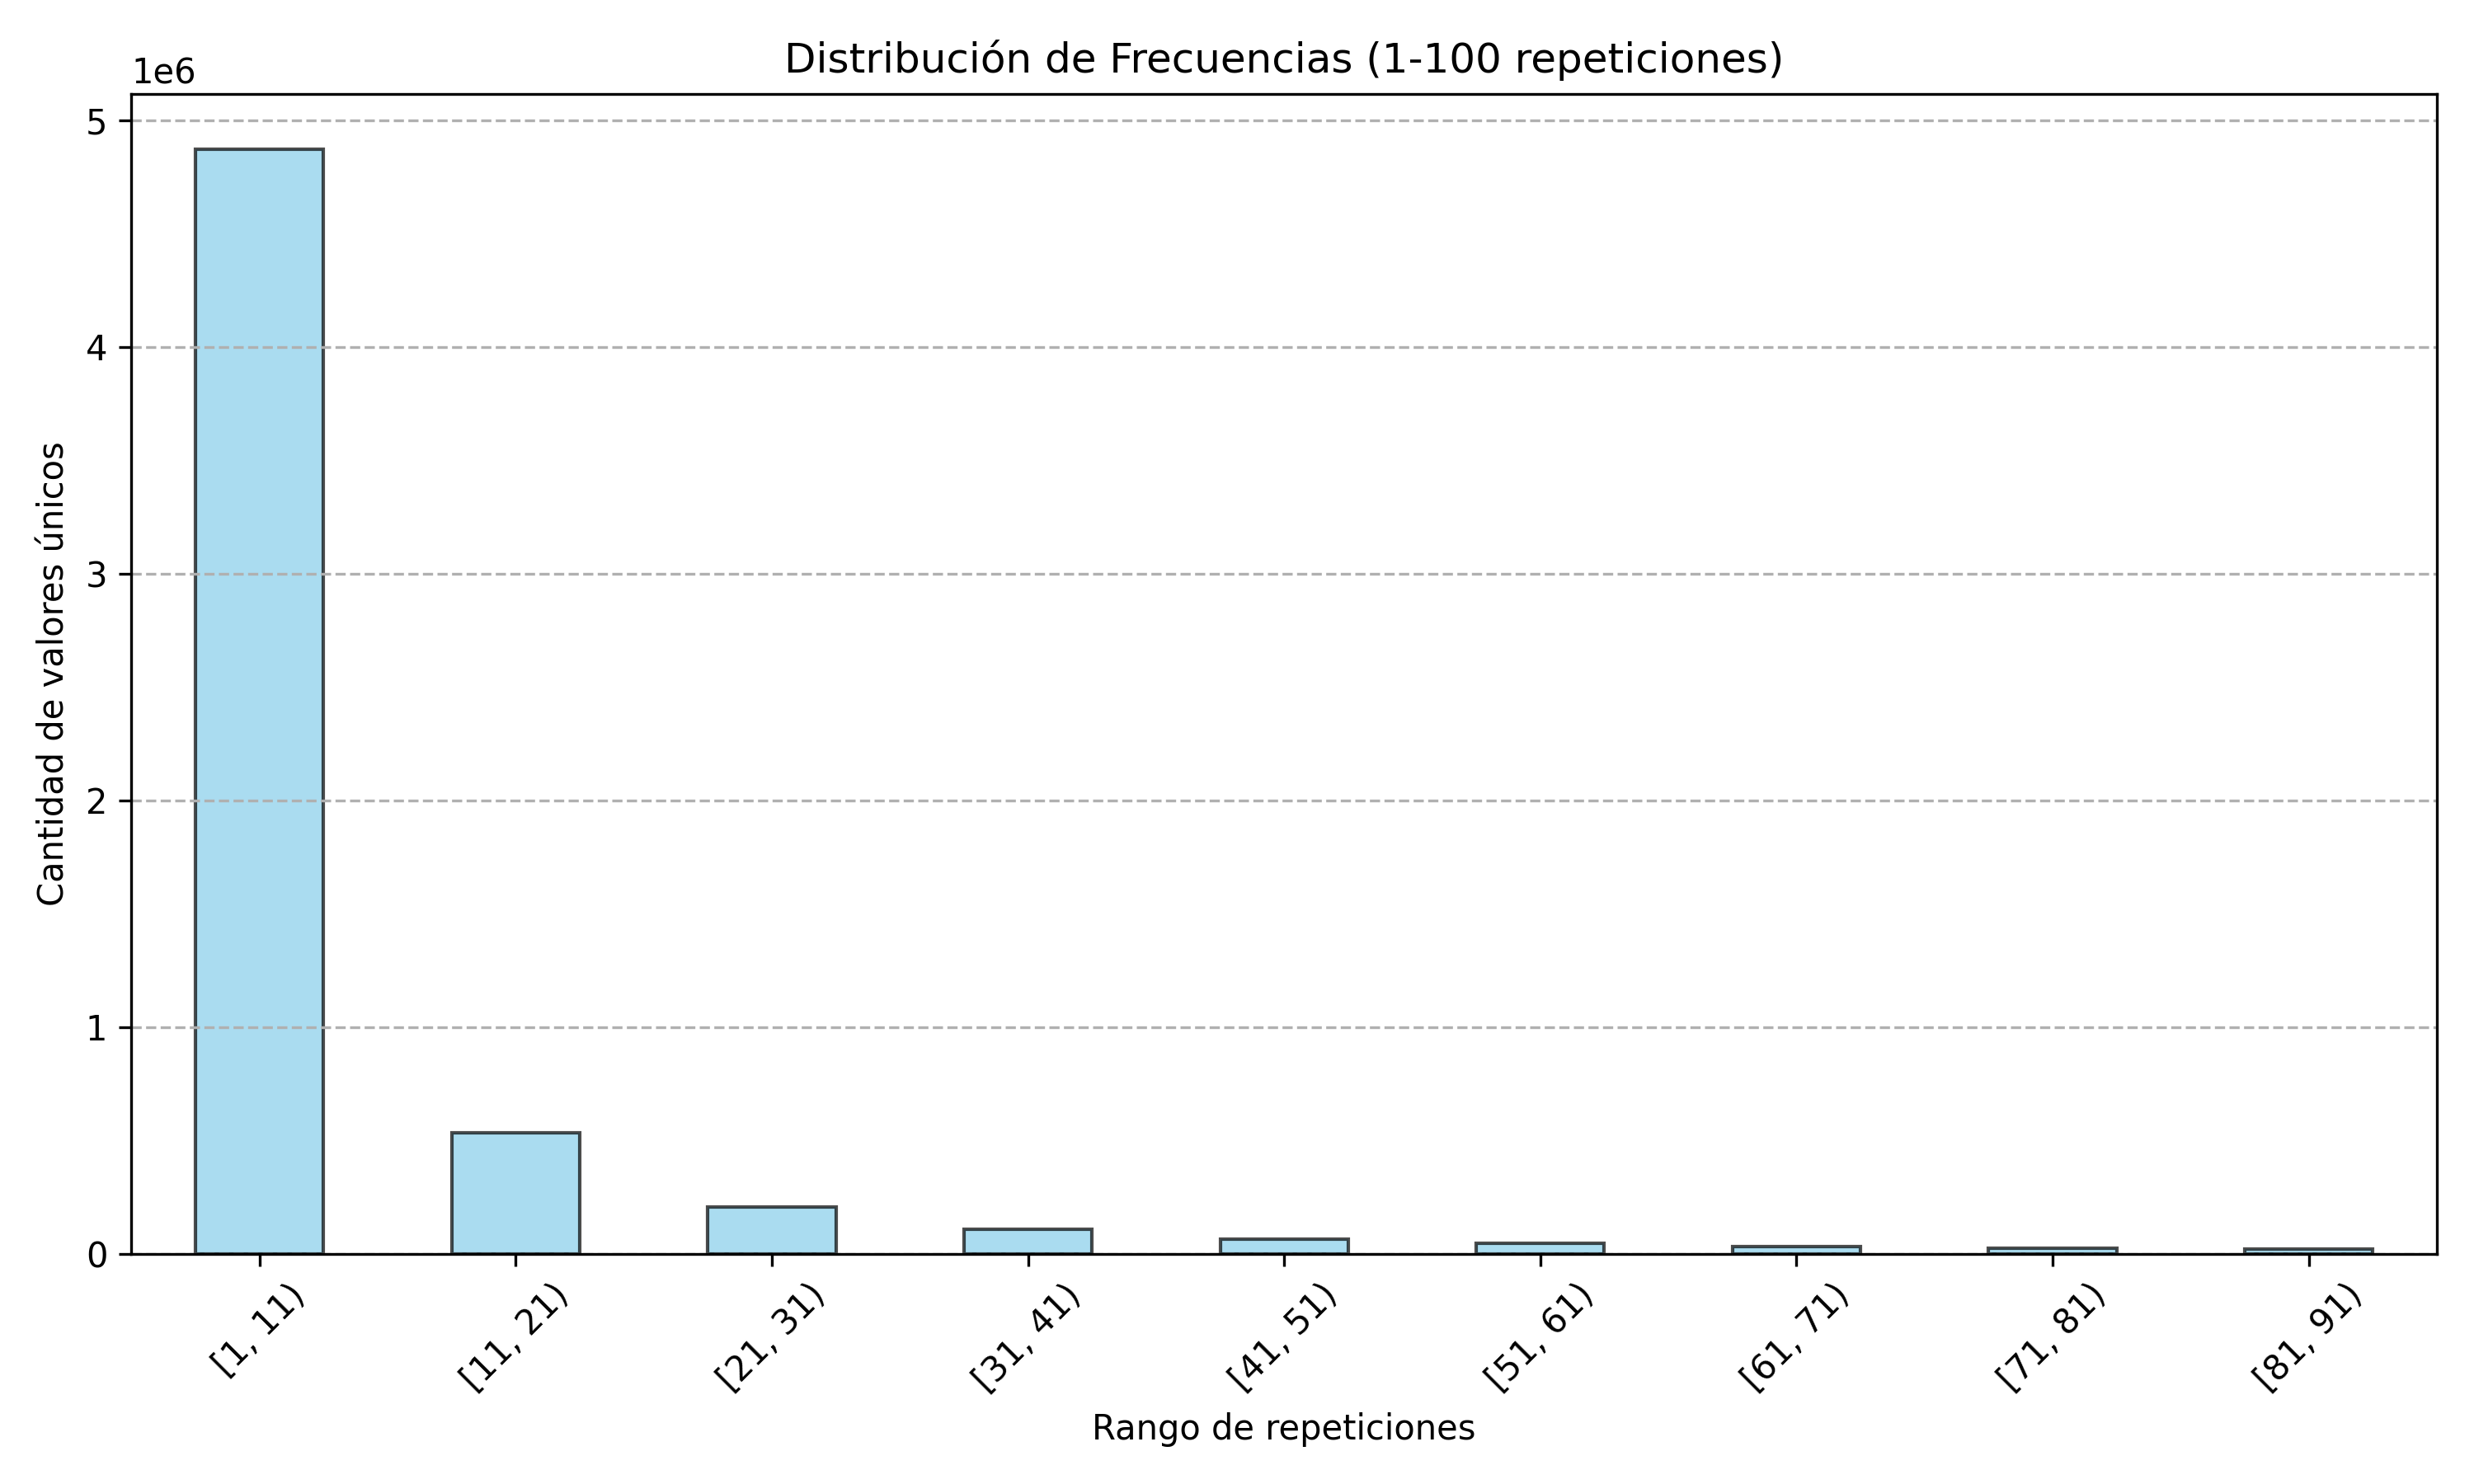
\includegraphics[width=\linewidth]{img/histograma_1_100.png}
        \caption{Histograma 1-100}
        \label{fig:sub1}
    \end{subfigure}
    \hfill % Espacio flexible y automático
    \begin{subfigure}[t]{0.48\textwidth-1em}
        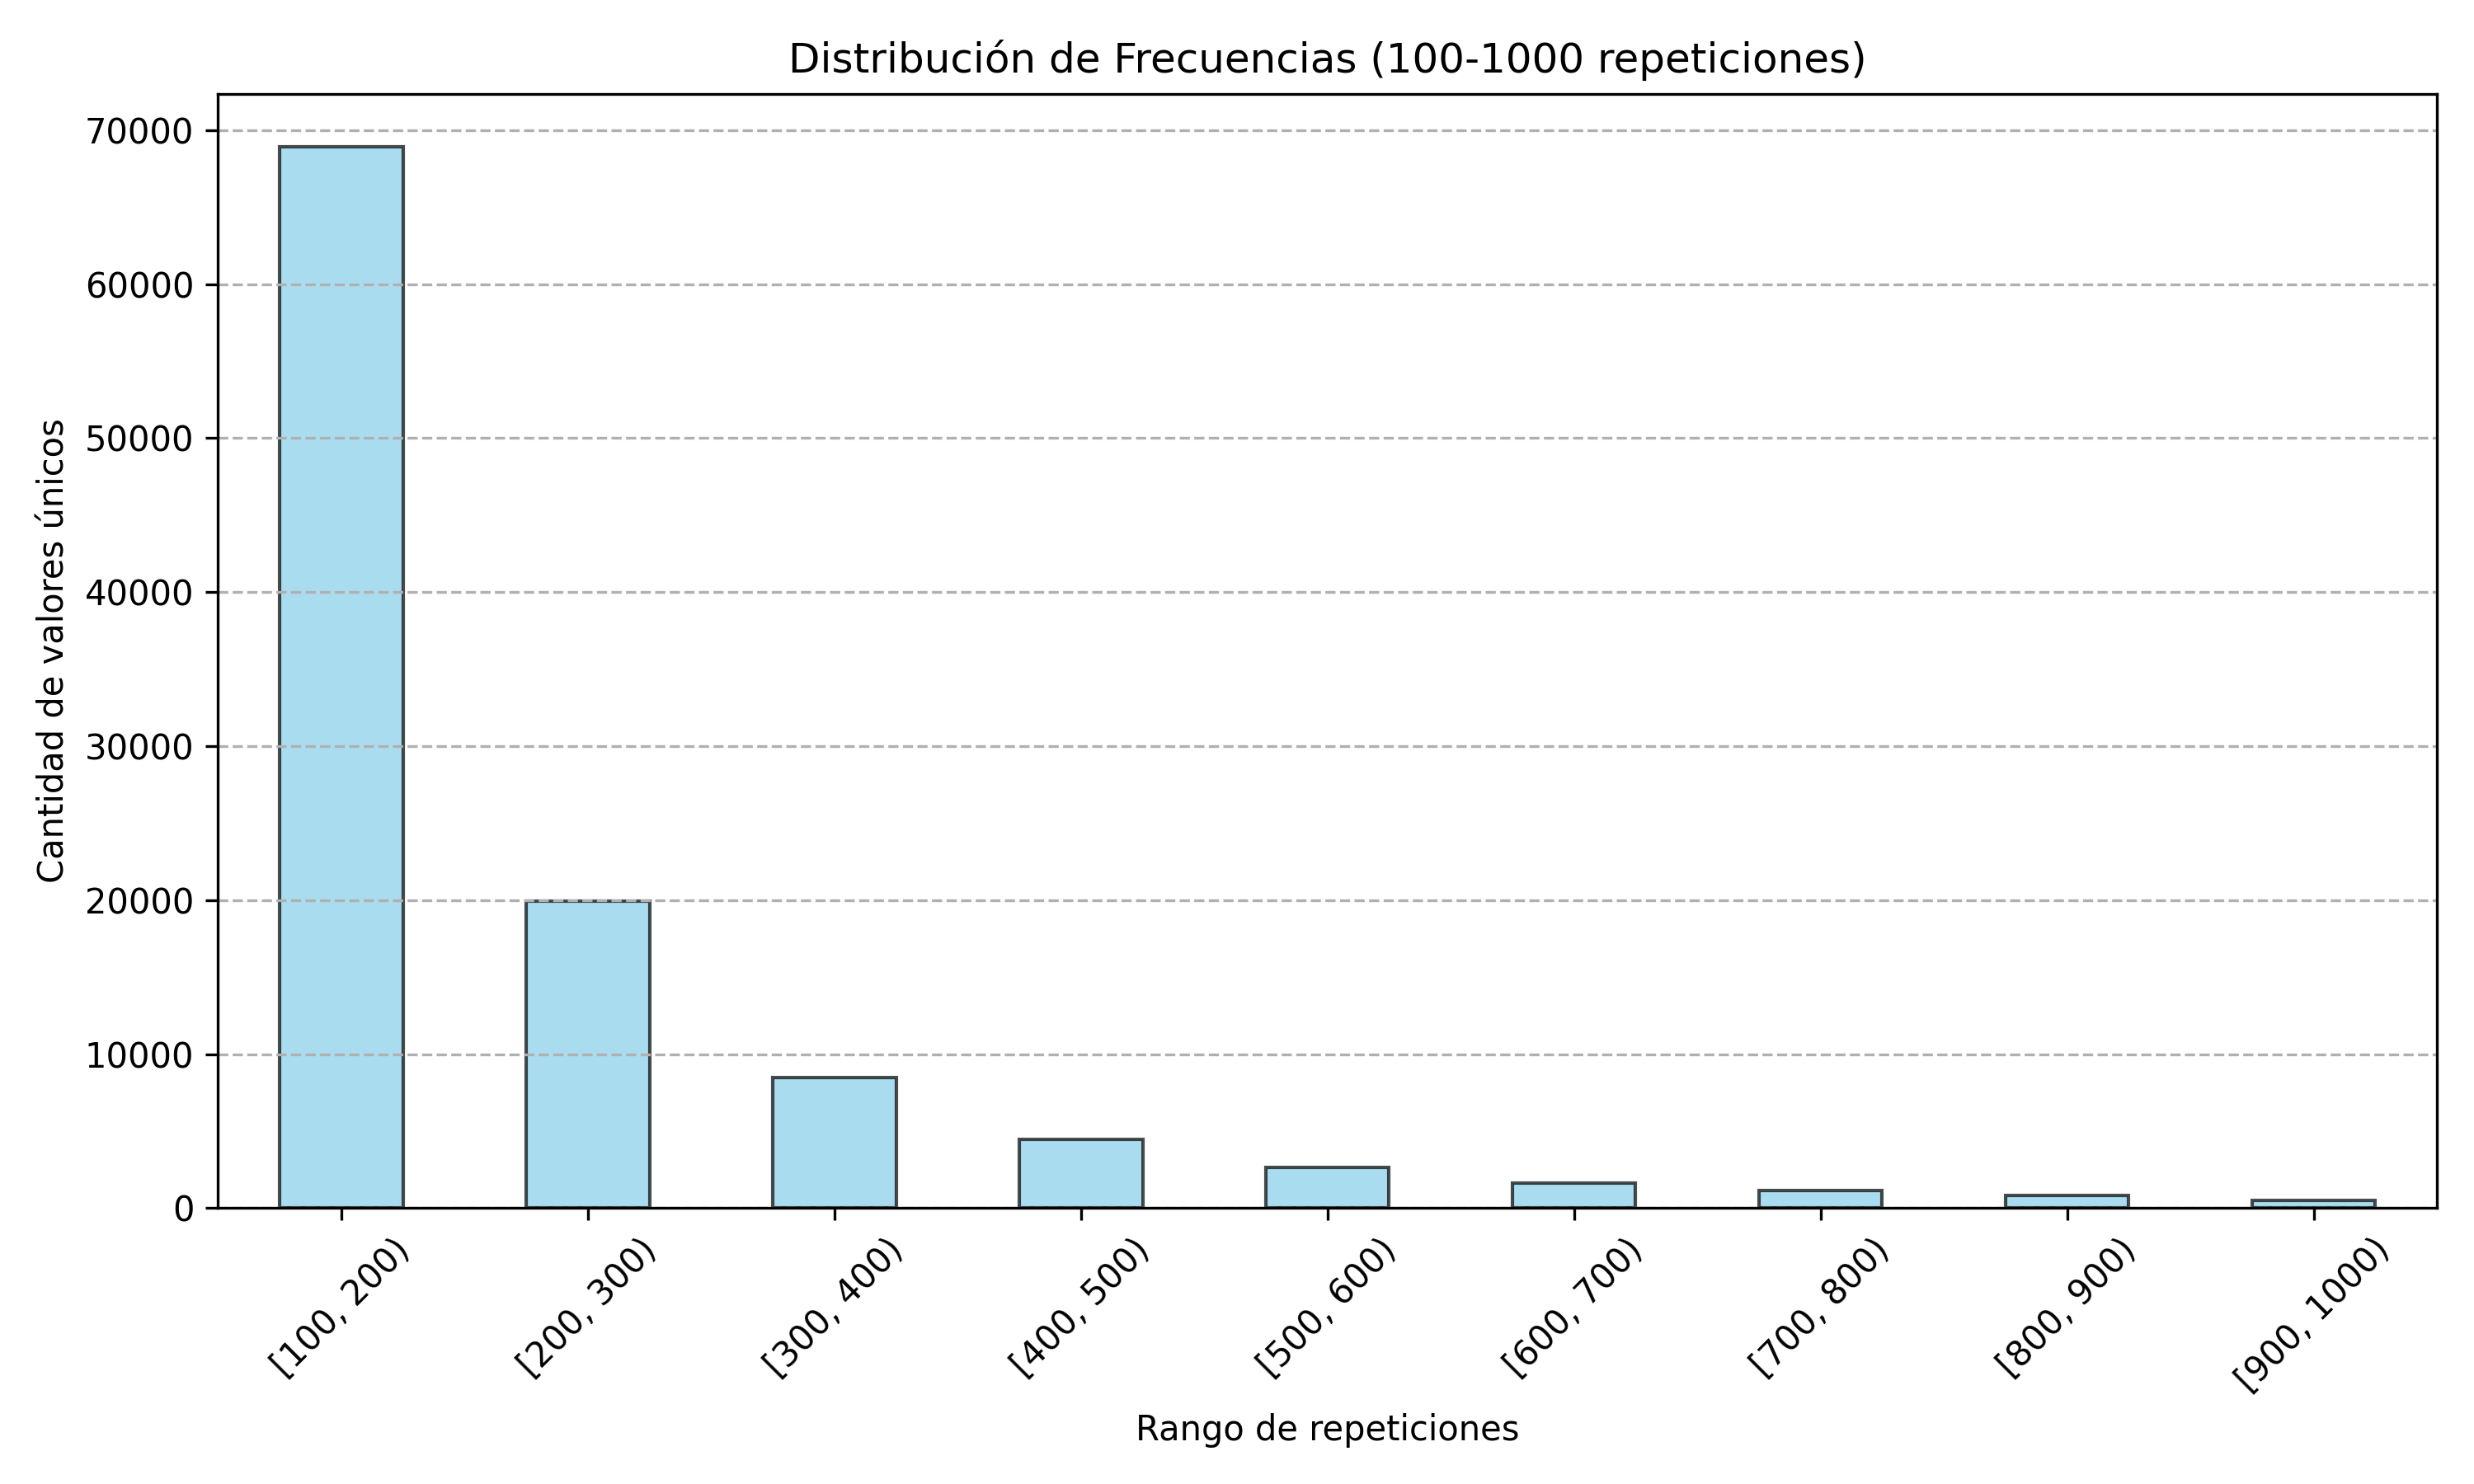
\includegraphics[width=\linewidth]{img/histograma_100_1000.png}
        \caption{Histograma 100-1000}
        \label{fig:sub2}
    \end{subfigure}

    \vspace{0.5cm} % Espacio entre las dos filas

    \begin{subfigure}[t]{0.48\textwidth}
        \centering
        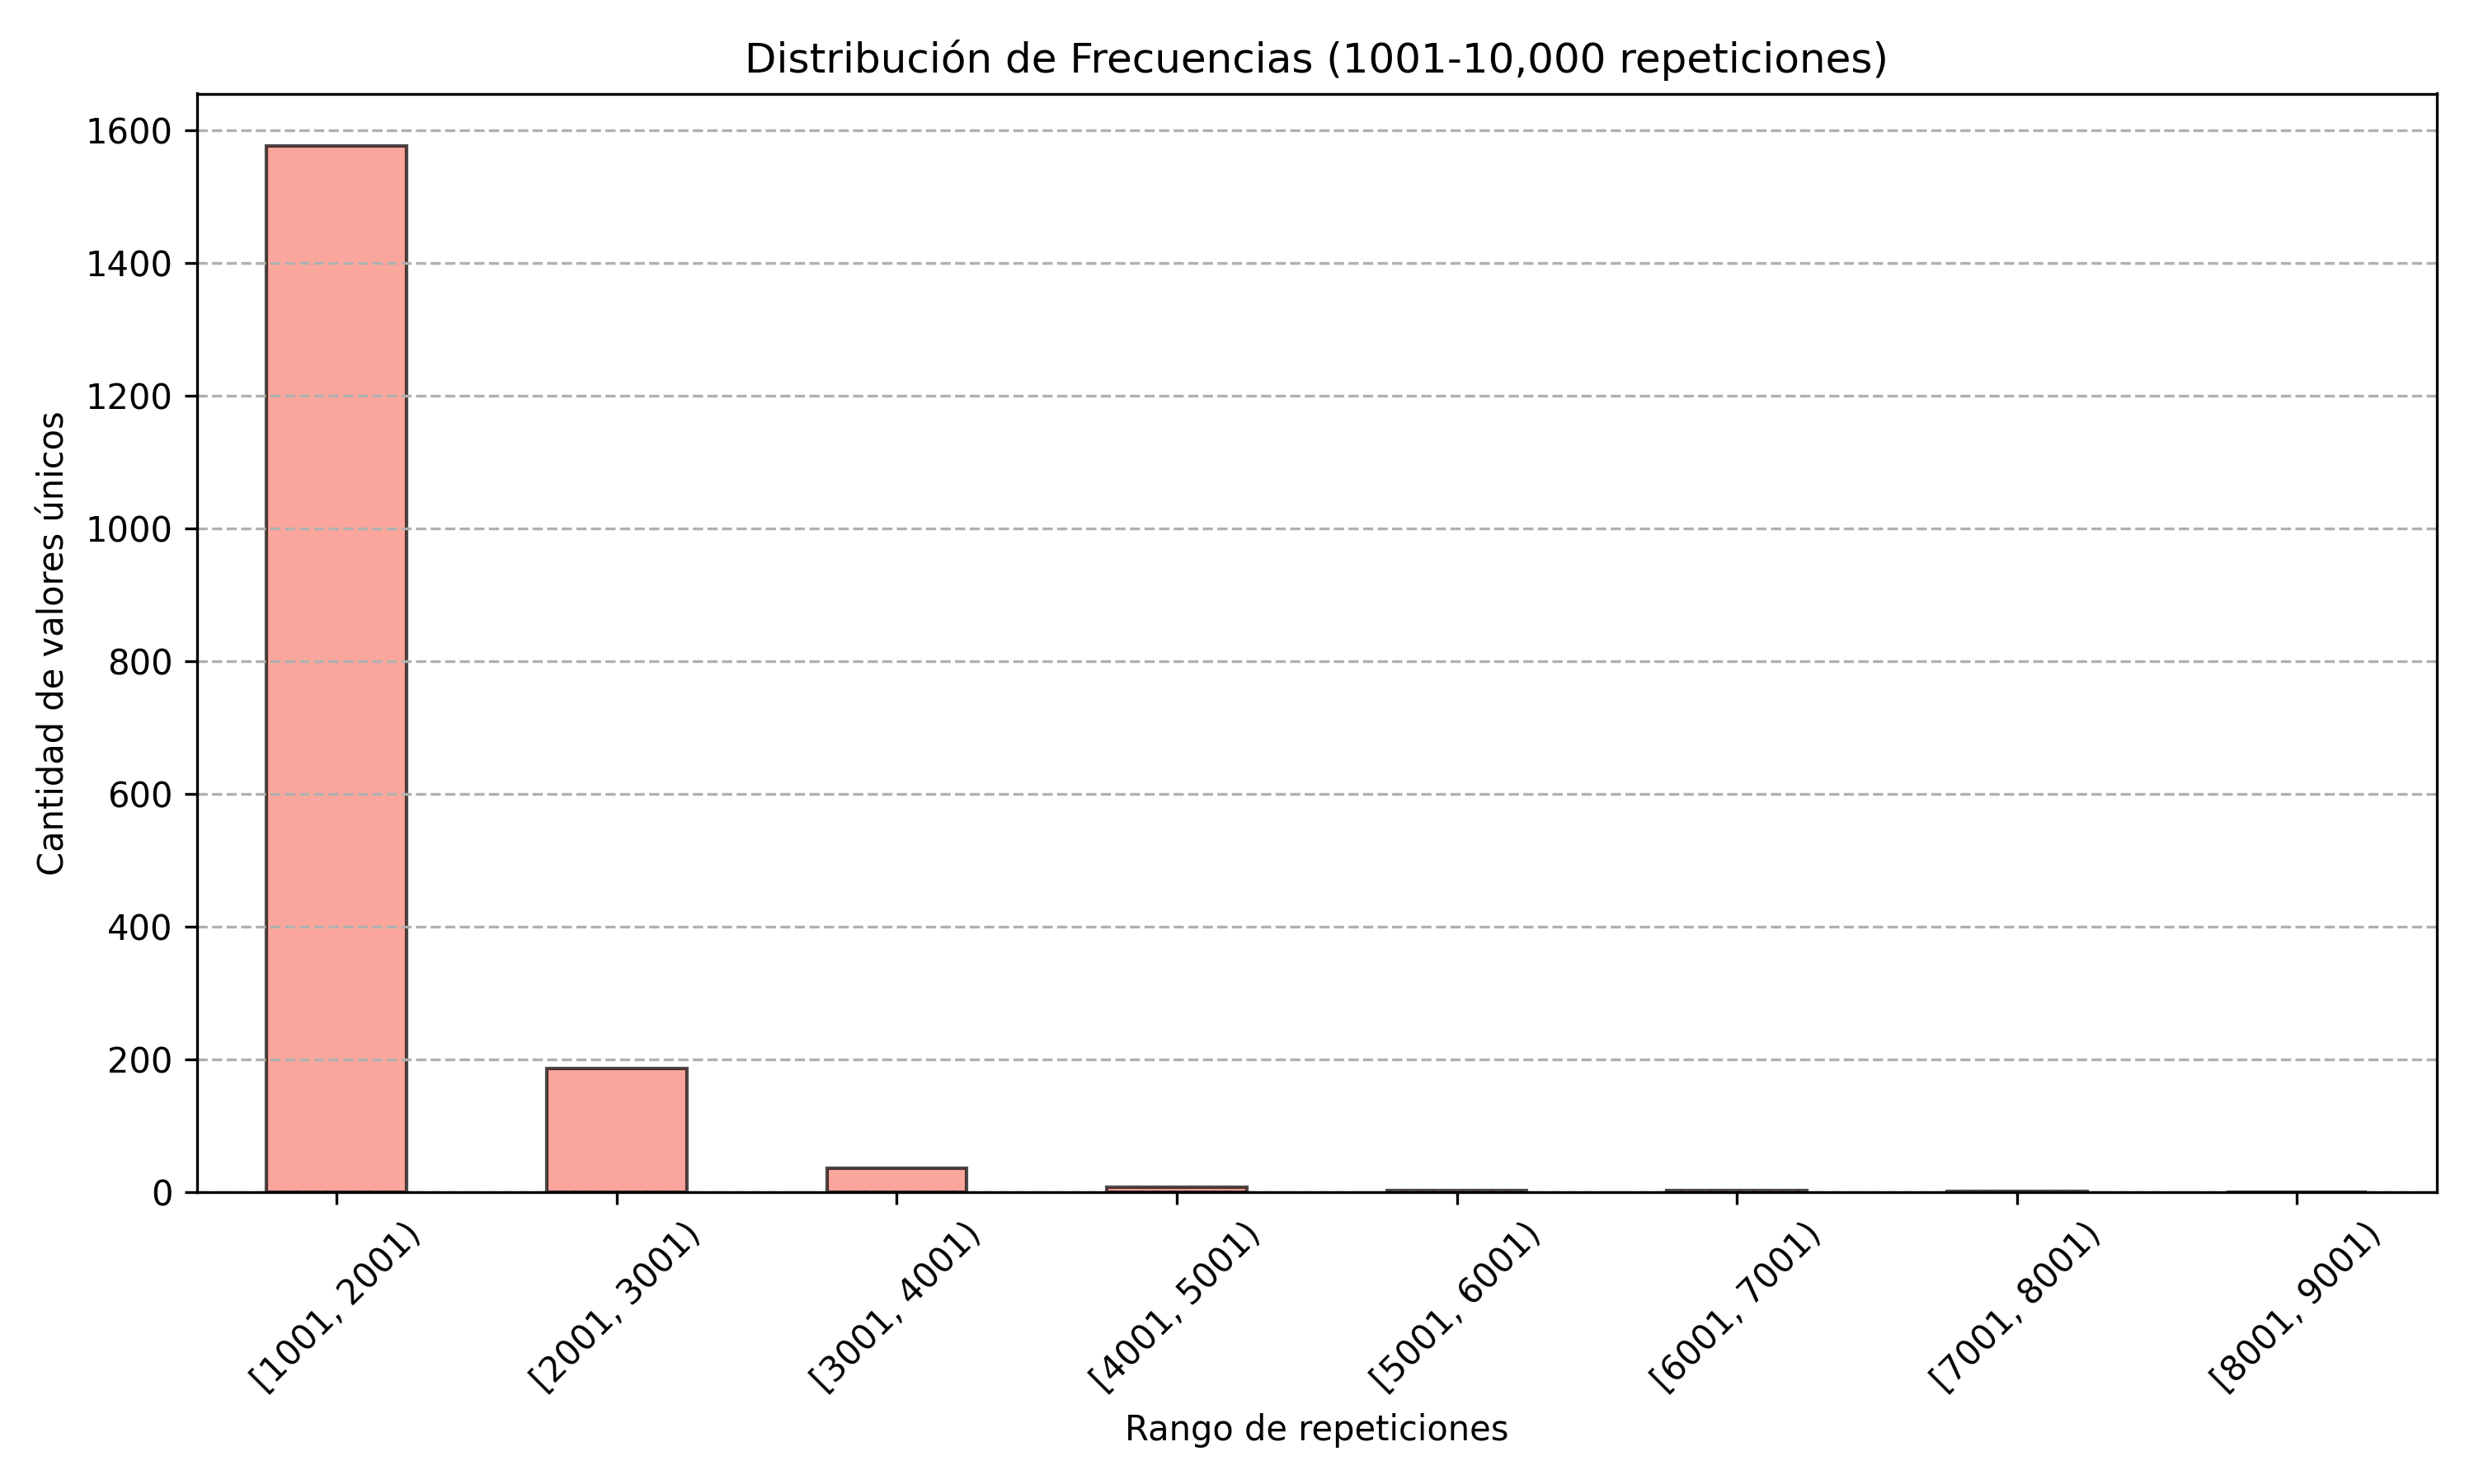
\includegraphics[width=\linewidth]{img/histograma_1001_10000.png}
        \caption{Histograma 1001-10000}
        \label{fig:sub3}
    \end{subfigure}

    \caption{Comparación de histogramas}
    \label{fig:histogramas}
\end{figure}

\noindent Además de los histogramas de la figura anterior el código también genera un resumen de las frecuencias de los valores únicos en cada rango. Este resumen se muestra a continuación:

\begin{verbatim}
        === Resumen de frecuencias ===
        **Rango 1-100 repeticiones**:
        - Total de valores unicos: 5,912,437

        **Rango 100-1000 repeticiones**:
        - Total de valores unicos: 108,519

        **Rango 1000-10000 repeticiones**:
        - Total de valores unicos: 1,816
\end{verbatim}

\noindent Gracias a esta información podemos observar que la mayoría de los identificadores únicos se encuentran en el rango de 1 a 100 repeticiones, dentro del cual la gran mayoría de ellos tienen entre una a diez repeticiones. Con base en podemos acotar los valores que serán considerados válidos para el análisis.

\begin{lstlisting}[
    language=Python,
    caption={identifier\_histogram\_detailed.py, análisis de frecuencias de la columna 'identifier'.},
    label={cod:identifier_histogram_detailed}
    ]
    import os
    import pandas as pd
    import matplotlib.pyplot as plt
    import numpy as np
    from collections import Counter

    archivo_csv = "Mobility_Data_Slim.csv"
    columna = "identifier"  
    chunksize = 1_000_000  
    os.makedirs("img", exist_ok=True)

    counter = Counter()
    for chunk in pd.read_csv(archivo_csv, usecols=[columna], chunksize=chunksize):
        counter.update(chunk[columna].dropna().astype(str))
    frecuencias = pd.Series(counter)

    frecuencias_bajas = frecuencias[(frecuencias >= 1) & (frecuencias <= 99)]
    frecuencias_medias = frecuencias[(frecuencias >= 100) & (frecuencias <= 1000)]
    frecuencias_altas = frecuencias[(frecuencias >= 1001) & (frecuencias <= 10000)]

    bins_bajas = list(range(1, 100, 10))  # 1-99 en pasos de 10 
    bins_medias = list(range(100, 1001, 100))  # 100-1000 en pasos de 100
    bins_altas = list(range(1001, 10001, 1000))  # 1001-10000 en pasos de 1000

    freciencias_bajas_agrupadas = pd.cut(frecuencias_bajas, bins=bins_bajas, right=False).value_counts().sort_index()
    frecuencias_medias_agrupadas = pd.cut(frecuencias_medias, bins=bins_medias, right=False).value_counts().sort_index()
    frecuencias_altas_agrupadas = pd.cut(frecuencias_altas, bins=bins_altas, right=False).value_counts().sort_index()

    print("\n=== Resumen de frecuencias ===")
    print(f"\n**Rango 1-100 repeticiones**:")
    print(f" - Total de valores unicos: {len(frecuencias_bajas)}")
    print(f"\n**Rango 100-1000 repeticiones**:")
    print(f" - Total de valores unicos: {len(frecuencias_medias)}")
    print(f"\n**Rango 1000-10000 repeticiones**:")
    print(f" - Total de valores unicos: {len(frecuencias_altas)}")


    plt.figure(figsize=(10, 6))
    freciencias_bajas_agrupadas.plot(kind='bar', color='skyblue', edgecolor='black', alpha=0.7)
    plt.title("Distribucion de Frecuencias (1-100 repeticiones)")
    plt.xlabel("Rango de repeticiones")
    plt.ylabel("Cantidad de valores unicos")
    plt.xticks(rotation=45)
    plt.grid(axis='y', linestyle='--')
    plt.tight_layout()
    plt.savefig(os.path.join("img", "histograma_1_100.png"), dpi=300)
    plt.close()

    plt.figure(figsize=(10, 6))
    frecuencias_medias_agrupadas.plot(kind='bar', color='skyblue', edgecolor='black', alpha=0.7)
    plt.title("Distribucion de Frecuencias (100-1000 repeticiones)")
    plt.xlabel("Rango de repeticiones")
    plt.ylabel("Cantidad de valores unicos")
    plt.xticks(rotation=45)
    plt.grid(axis='y', linestyle='--')
    plt.tight_layout()
    plt.savefig(os.path.join("img", "histograma_100_1000.png"), dpi=300)
    plt.close()

    plt.figure(figsize=(10, 6))
    frecuencias_altas_agrupadas.plot(kind='bar', color='salmon', edgecolor='black', alpha=0.7)
    plt.title("Distribucion de Frecuencias (1001-10,000 repeticiones)")
    plt.xlabel("Rango de repeticiones")
    plt.ylabel("Cantidad de valores unicos")
    plt.xticks(rotation=45)
    plt.grid(axis='y', linestyle='--')
    plt.tight_layout()
    plt.savefig(os.path.join("img", "histograma_1001_10000.png"), dpi=300)
    plt.close()

    print("Graficos guardados en /img/")
    
\end{lstlisting}

\subsection{Identificar y manejar valores faltantes o nulos en el conjunto de datos}

